\ProvidesFile{section_3_complex_numbers}[Section 3]

\newpage

\section{Complex numbers}
\subsection{Why do we need complex numbers?}

\begin{example}
We need complex numbers because they allow us to find the roots of every polynomial equation with real coefficients, even equations like $x^2 + 1 = 0$ (see exercise \ref{roots_of_x2_1}).  These roots are then used to study matrices of linear operators during the course.
\end{example}

\begin{example} Sometimes complex numbers help us find real roots of polynomial equations. This is particularly true for third-degree equations, as shown in \href{https://en.wikipedia.org/wiki/Cubic_equation#General_cubic_formula}{Cardano's formula}. If we closely analyze the formula, we can observe that even in cases where the roots are real, we may need to extract square roots of negative numbers at some point during the calculation.
\end{example}

\begin{example}
Complex numbers are used in signal processing, where they help study periodic functions like $\sin(\omega t)$ and $\cos(\omega t)$, since $e^{i\omega t} = \cos(\omega t) + i\sin(\omega t)$.
\end{example}

\begin{example}
Complex numbers are widely used in quantum computing, and without them, it would be impossible to construct and use a quantum computer.
\end{example}

\subsection{Field of complex numbers}

For some reason we will describe later (see theorem \ref{c_field}), we will call the set of complex numbers a field.

\begin{definition}\label{complex}
The field of \underline{\it complex numbers}, denoted by $\C$, is the set of all ordered pairs of real numbers
$$\R^2 = \R\times\R = \{(a,b) \mid a,b \in \R\}$$
with addition and multiplication defined as follows:
$$
(a, b)+(c, d)=(a+c, b+d)\text{ for all }(a, b),~(c, d) \in \R^2,$$
$$(a, b) \cdot(c, d)=(a c-b d, a d+b c)\text{ for all }(a, b),~(c, d) \in \R^2.$$
\end{definition}

\begin{theorem}\label{complex_properties}
$\C$ from definition \ref{complex} satisfies the following properties:

1) For any $(a, b),(c, d) \in \R^2$, we have $(a, b)+(c, d) = (c, d)+(a, b)$ (addition is commutative);

2) For any $(a, b),(c, d),(e, f) \in \R^2$, we have $((a, b)+(c, d))+(e, f) = (a, b)+((c, d)+(e, f))$ (addition is associative);

3) There exists $0=(0,0)\in\C$ such that for any $(a, b) \in \R^2$, we have $(0,0)+(a, b) = (a, b)$ (existence of additive identity);

4) For any $(a, b) \in \R^2$ there exists $-(a, b) = (-a,-b)$, such that $(a, b)+(-(a, b)) = (0,0)$ (existence of additive inverse);

5) For any $(a, b),(c, d),(e, f) \in \R^2$, we have $(a, b) \cdot((c, d)+(e, f)) = (a, b) \cdot(c, d)+(a, b) \cdot(e, f)$ (multiplication is distributive over addition);

6) For any $(a, b),(c, d) \in \R^2$, we have $(a, b) \cdot(c, d) = (c, d) \cdot(a, b)$ (multiplication is commutative);

7) For any $(a, b),(c, d),(e, f) \in \R^2$, we have $(a, b) \cdot((c, d) \cdot(e, f)) = ((a, b) \cdot(c, d)) \cdot(e, f)$ (multiplication is associative);

8) There exists $1=(1,0)\in\C$ such that for any $(a, b) \in \R^2$, we have $(1,0) \cdot(a, b) = (a, b)$ (existence of multiplicative identity);

9) For any $(a, b) \in \R^2 \backslash\{(0,0)\}$ there exists $(a, b)^{-1} = \left(\frac{a}{a^2+b^2}, \frac{-b}{a^2+b^2}\right)$, such that $(a, b) \cdot(a, b)^{-1} = (1,0)$ (existence of multiplicative inverse).
\end{theorem}

\begin{proof}
Check all conditions from the definition:

1) For any $(a, b),(c, d) \in \R^2$, we have:
$$
\begin{aligned}
(a, b)+(c, d) & =(a+c, b+d) \\
& =(c+a, d+b) \\
& =(c, d)+(a, b) .
\end{aligned}
$$

2) For any $(a, b),(c, d),(e, f) \in \R^2$, we have:
$$
\begin{aligned}
((a, b)+(c, d))+(e, f) & =(a+c, b+d)+(e, f) \\
& =((a+c)+e,(b+d)+f) \\
& =(a+(c+e), b+(d+f)) \\
& =(a, b)+(c+e, d+f) \\
& =(a, b)+((c, d)+(e, f)) .
\end{aligned}
$$

3) Let $\mathbb{C} \ni 0 = (0,0) \in \R^2$, then for any $(a, b) \in \R^2$, we have:
$$
\begin{aligned}
(0,0)+(a, b) & =(0+a, 0+b) \\
& =(a, b) .
\end{aligned}
$$

4) For any $(a, b) \in \R^2$ let $-(a, b) = (-a,-b)$, then
$$
\begin{aligned}
(a, b)+(-(a, b)) & =(a, b)+(-a,-b) \\
& =(a+(-a), b+(-b)) \\
& =(0,0) .
\end{aligned}
$$

5) For any $(a, b),(c, d),(e, f) \in \R^2$, we have:
$$
\begin{aligned}
(a, b) \cdot((c, d)+(e, f)) & =(a, b) \cdot(c+e, d+f) \\
& =(a(c+e)-b(d+f), a(d+f)+b(c+e)) \\
& =(a c+a e-b d-b f, a d+a f+b c+b e) \\
& =(a c-b d+a e-b f, a d+b c+a f+b e) \\
& =(a c-b d, a d+b c)+(a e-b f, a f+b e) \\
& =(a, b) \cdot(c, d)+(a, b) \cdot(e, f) .
\end{aligned}
$$

6) For any $(a, b),(c, d) \in \R^2$, we have:
$$
\begin{aligned}
(a, b) \cdot(c, d) & =(a c-b d, a d+b c) \\
& =(c a-d b, c b+d a) \\
& =(c, d) \cdot(a, b) .
\end{aligned}
$$

7) For any $(a, b),(c, d),(e, f) \in \R^2$, we have:
$$
\begin{aligned}
(a, b) \cdot((c, d) \cdot(e, f)) & =(a, b) \cdot(c e-d f, c f+d e) \\
& =(a(c e-d f)-b(c f+d e), a(c f+d e)+b(c e-d f)) \\
& =(a c e-a d f-b c f-b d e, a c f+a d e+b c e-b d f) \\
& =(a c e-b d e-a d f-b c f, a c f-b d f+a d e+b c e) \\
& =((a c-b d) e-(a d+b c) f,(a c-b d) f+(a d+b c) e) \\
& =(a c-b d, a d+b c) \cdot(e, f) \\
& =((a, b) \cdot(c, d)) \cdot(e, f) .
\end{aligned}
$$

8) Let $\mathbb{C} \ni 1 = (1,0) \in \R^2$, then for any $(a, b) \in \R^2$, we have:
$$
\begin{aligned}
(1,0) \cdot(a, b) & =(1 a-0 b, 1 b+0 a) \\
& =(a, b) .
\end{aligned}
$$

9) For any $(a, b) \in \R^2 \backslash\{(0,0)\}$ let $(a, b)^{-1} = \left(\frac{a}{a^2+b^2}, \frac{-b}{a^2+b^2}\right)$, then
$$
\begin{aligned}
(a, b) \cdot(a, b)^{-1} & =(a, b) \cdot\left(\frac{a}{a^2+b^2}, \frac{-b}{a^2+b^2}\right) \\
& =\left(\frac{a^2}{a^2+b^2}-\frac{b(-b)}{a^2+b^2}, \frac{a(-b)}{a^2+b^2}+\frac{b a}{a^2+b^2}\right) \\
& =(1,0) .
\end{aligned}
$$
\end{proof}

We can identify the subset $S=\{(a, 0) \mid a \in \R\} \subset \R^2$ with real numbers. Indeed, if $a\in\R$ corresponds to $(a, 0)$, then addition and multiplication of these complex numbers work as in the reals: 

$$
\begin{aligned}
(a, 0)+(b, 0) & =(a+b, 0)\\
(a, 0) \cdot(b, 0) & =\left(a b-0^2, a 0+0 b\right)=(a b, 0).
\end{aligned}
$$

\begin{definition}
The element $(0, 1)\in \C$ is called \underline{\it the imaginary unit} and denoted $i = (0, 1)$.
\end{definition}

\begin{exercise}
Prove that $i^2 = -1 = (-1, 0)$.
\end{exercise}

\begin{exercise}\label{roots_of_x2_1}
Prove that the equation $x^2 + 1 = 0$ has exactly two solutions $\pm i$ in $\C$.
\end{exercise}

\begin{center}
    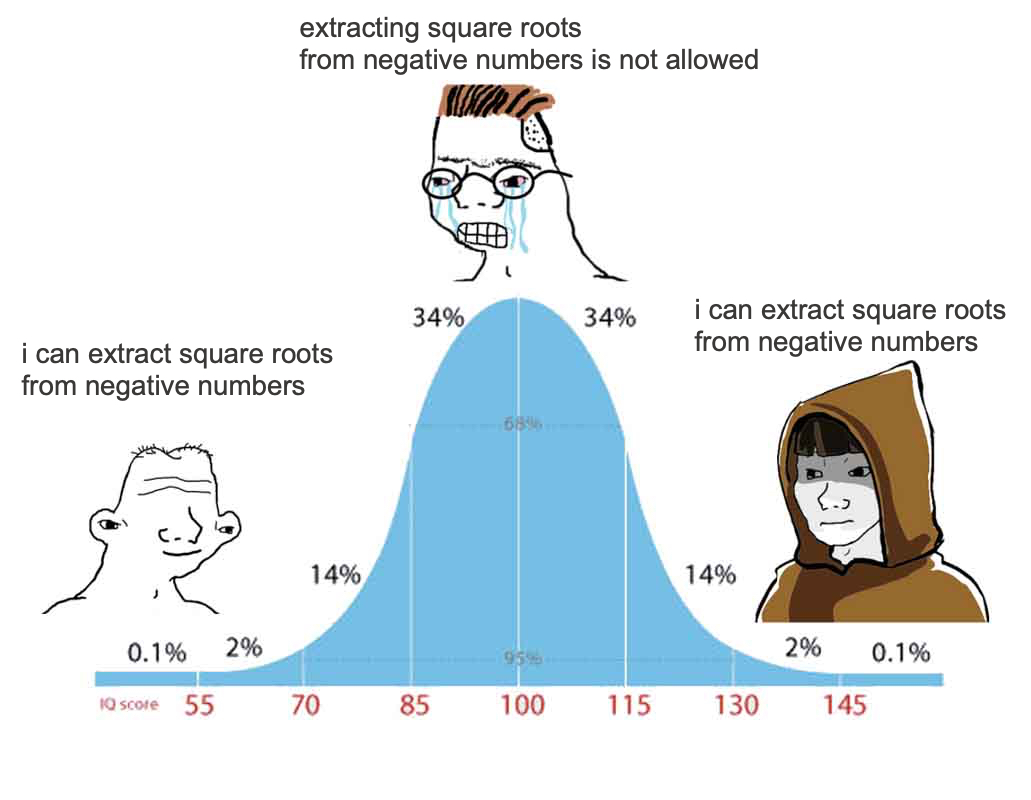
\includegraphics[scale=0.2]{Images/roots meme.jpeg}
\end{center}

\begin{definition}
The representation $z=(a, b)$ is called the \underline{\it Cartesian form} of a complex number $z$ (named after René Descartes, {\it lat.} Renatus Cartesius).
\end{definition}

\begin{lemma}
Any complex number $z=(a, b)$ can be uniquely represented in the form $z = a + bi$.
\end{lemma} 

\begin{proof}
Since $i = (0,1)$, we have $z=(a, b)=(a, 0)+(b, 0) \cdot(0,1)=a+b i$, so the representation exists.
    
If $a+b i=a^{\prime}+b^{\prime} i$ then
$$
(a, b)=(a, 0)+(b, 0) \cdot(0,1)=a+b i=a^{\prime}+b^{\prime} i=\left(a^{\prime}, 0\right)+\left(b^{\prime}, 0\right) \cdot(0,1)=\left(a^{\prime}, b^{\prime}\right) .
$$
By the definition of ordered pair, from the equality $(a, b)=\left(a^{\prime}, b^{\prime}\right)$ we have $a=a^{\prime}$ and $b=b^{\prime}$, so the representation is unique.
\end{proof}

\begin{definition}
The form $a + bi$ is called the \underline{\it algebraic form} of a complex number $z$.
\end{definition}

\begin{exercise}
Check that all properties from theorem \ref{complex_properties} hold true in algebraic form.  
\end{exercise}

\begin{definition}
Let $z=a+b i$ be a complex number, then the \underline{\it real part} of $z$ is
$$
\Re(z) = \Re(a+bi) = a,
$$
and the imaginary part of $z$ is
$$
\Im(z) = \Im(a+bi) = b.
$$
\end{definition}

\begin{remark}
Both $\Re(z)$ and $\Im(z)$ are real and $\Re(z) + i\Im(z) = z$ for any complex number $z$.
\end{remark}

% TODO: show coordinates on the complex plane

\begin{definition}
The \underline{\it absolute value} (or \underline{\it modulus}) of a complex number $z=a+b i$ is
$$
|z| = \sqrt{a^2+b^2} .
$$
\end{definition}

\begin{remark} For real numbers, the absolute value in the real and complex senses is the same.
\end{remark}

\begin{exercise}
    Find $|z|$ where $z = 1, i, -i, 1+i$.
    \end{exercise}

\subsection{Geometric interpretation}

In the geometric interpretation, a complex number $ z = a+bi$ is represented as a vector in a Cartesian coordinate system, extending from the point $(0, 0)$ to the point $(a, b) = (\Re(z), \Im(z))$.

The addition of complex numbers corresponds to the addition of vectors.

\begin{exercise}
Prove that complex numbers form a vector space over the real numbers. Find a basis and the dimension of this vector space.
\end{exercise}

\subsection{* Fields}

\begin{definition}
A \underline{\it binary operation} on a set $S$ is a \underline{mapping} of the elements of the \underline{Cartesian product} $S \times S$ to $S$:
$$
f \colon S \times S \rightarrow S.
$$
\end{definition}

\begin{definition}
A \underline{\it field} is a triple $(F,+, \cdot)$, where $F$ is a set, and 
$$+\colon F \times F \rightarrow F,$$
$$\cdot\colon F \times F \rightarrow F$$
are binary operations (written $(a, b) \mapsto a+b$ and $(a, b) \mapsto a \cdot b$ and called addition and multiplication, respectively) such that the following conditions are satisfied for any $a, b, c \in F$:
\begin{enumerate}
    \item $a+b = b+a$ (commutativity of addition),
    \item $(a+b)+c = a+(b+c)$ (associativity of addition),
    \item $0 \in F$ such that $0+a=a$ (existence of additive identity),
    \item for any $a \in F$ there is $-a \in F$ such that $a+(-a)=0$ (existence of additive inverse),
    \item $a \cdot b=b \cdot a$ (commutativity of multiplication),
    \item $(a \cdot b) \cdot c =a \cdot(b \cdot c)$ (associativity of multiplication),
    \item there is $1 \in F \backslash\{0\}$ such that $1 \cdot a=a$ (existence of multiplicative identity),
    \item if $a \in F \backslash\{0\}$ then there is $a^{-1} \in F$ such that $a \cdot a^{-1}=1$ (existence of multiplicative inverse), 
    \item $a\cdot(b+c) =a\cdot b+a\cdot c$ (distributivity of multiplication over addition).
\end{enumerate}
\end{definition}

\begin{remark}
We normally omit the multiplication sign $\cdot$, especially when it is clear from the context.
\end{remark}

\begin{example}
    \begin{itemize}
        \item[a) ] $\R$ --- field of real numbers, operations: regular addition and multiplication of numbers,
        \item[b) ] $\Q$ --- field of rationals, operations are the same,
        \item[c) ] $\F_2 = (\{0, 1\},~ +_{\mod 2},~ \cdot_{\mod 2})$.
    \end{itemize}
\end{example}

\begin{exercise}
    Check that fields from the previous example a), b), c) are actually fields. Build addition and multiplication tables for $\F_2$.
\end{exercise}

\begin{theorem}\label{c_field}
$\C$ from definition \ref{complex} is actually a field.
\end{theorem}

\begin{proof}
    Follows immediately from theorem \ref{complex_properties}.
\end{proof}

\begin{exercise}
    Let $\F$ be a field. Prove that
    \begin{itemize}
        \item [a) ] the additive identity $0\in \F$ is unique;
        \item [b) ] the multiplicative identity of $1\in \F$ is unique;
        \item [c) ] $\forall x\in \F~\exists !~-x\in \F$ (the additive inverse is unique for every field element);
        \item [d) ] $\forall x\in\F\backslash\{0\}~\exists ! ~x^{-1}\in\F$;
        \item [e) ] $\forall x\in \F ~x\cdot 0 = 0\cdot x = 0$;
        \item [f) ] $\forall x\in \F ~(-1) \cdot x=x\cdot(-1)=-x $.
    \end{itemize}
\end{exercise}

\begin{definition}
 If $\F=(F,+, \cdot)$ is a field and a subset $S$ of $F$ satisfies conditions 1)--9) from the definition of a field with the same operations as in $\F$, then $\mathbb{S}=(S,+, \cdot)$ is called a subfield of $\mathbb{F}$.
\end{definition}

\begin{example}
$\Q$ is a subfield of $\R$.        
\end{example}

\begin{lemma}
Let $S=\{(a, 0) \mid a \in \R\} \subset \R^2$. Then $S$, with the operations inherited from $\C$, $(S,+, \cdot)$, is a subfield of $\mathbb{C}$, isomorphic to $\R$.
\end{lemma}

\subsection{Complex conjugate}

\begin{definition}
The \underline{\it complex conjugate} of a complex number $z=a+b i$, denoted $\bar{z}$, is defined to be
$$
\bar{z} = a-b i .
$$
\end{definition}

The geometric interpretation of complex conjugation is reflection with respect to the $x$-axis.

\begin{theorem}\label{conj}
For any $z, z_1, z_2 \in \mathbb{C}$, the complex conjugate satisfies the following properties:
\begin{enumerate}
\item $\overline{z_1+z_2}=\overline{z_1}+\overline{z_2}$;
\item $\overline{z_1 \cdot z_2}=\overline{z_1} \cdot \overline{z_2}$;
\item $(\bar{z}=z) \Leftrightarrow(\operatorname{Im}(z)=0)$;
\item $|\bar{z}|=|z|$;
\item $\overline{\bar{z}}=z$;
\item $\bar{z} \cdot z=|z|^2$.
\end{enumerate}
\end{theorem}

\begin{exercise}
Prove theorem \ref{conj}.
\end{exercise}

\begin{exercise}
Prove that:
\begin{enumerate}[a)]
\item a complex number $z$ is real if and only if $\overline{z} = z$;
\item a nonzero complex number $z$ is purely imaginary if and only if $\overline{z} = -z$.
\end{enumerate}
\end{exercise}

\begin{exercise}
Prove that if $z$ is a root of a polynomial with real coefficients, then its complex conjugate $\overline{z}$ is also a root of the polynomial.
\end{exercise}

\begin{exercise}
Prove that every real polynomial can be represented as a product of linear polynomials with real coefficients and quadratic polynomials with real coefficients and negative discriminant.
\end{exercise}

\subsection{Polar coordinates}
Each point in the plane $(a, b)$, except for the origin $(0, 0)$, 
is uniquely determined by its polar coordinates $(r, \varphi)$, where $r$ represents the distance from the point to the origin, 
and $\varphi$ is the angle between the positive x-axis and the radius vector of the point $(a, b)$, measured counterclockwise. The angle is determined up to an integer multiple of $2\pi$, i.e., $2\pi k$ with $k\in\Z$. This angle is referred to as the {\it argument} of the point.

Note that for the point $(0, 0)$ the argument is undefined.

\begin{exercise}
Find the coordinate transformation formulas from Cartesian to polar coordinates and vice versa.
\end{exercise}

Since there is a correspondence between complex numbers and points in $\R^2$, where a complex number $a + bi$ corresponds to the point $(a, b)$, we can utilize polar coordinates to analyze problems involving complex numbers. By doing so, we can use geometric concepts to resolve algebraic problems regarding complex numbers, and vice versa. In this context, we define the argument of a complex number $a+bi$ as the argument of the corresponding point $(a, b)$ and denote it $\arg(a+bi)$. 

Note that with this definition, the argument of a complex number is not uniquely determined.

\subsection{Absolute value properties}
\begin{lemma}
\begin{enumerate}
\item $\forall z, w\in\C ~|zw| = |z||w|$,
\item $\forall z\in \C\backslash\{0\} ~ |z^{-1}| = |z|^{-1}$,
\item $\forall z\in\C, w\in\C\backslash\{0\} ~\left|\frac{z}{w}\right| = \frac{|z|}{|w|}$.
\end{enumerate}
\end{lemma}

\begin{proof}
\begin{enumerate}
\item By lemma \ref{conj}, we have
$$
|zw| = \sqrt{(zw)\overline{(zw)}} = \sqrt{zw\overline{z}\overline{w}} =
\sqrt{z\bar{z}}\sqrt{w\bar{w}} = |z||w|.
$$
\item $1 = |1| = |z z^{-1}| = |z| |z^{-1}|$, then $|z^{-1}| = \frac{1}{|z|}$.
\item $\left|\frac{z}{w}\right| = |zw^{-1}| = |z||w^{-1}| = |z||w|^{-1} = \frac{|z|}{|w|}.$
\end{enumerate}
\end{proof}

\begin{lemma}
$\forall z, w\in\C ~|z + w|\leqslant |z| + |w|$.
\end{lemma}

\begin{proof} Using the geometric interpretation of complex numbers and their sums,
consider a triangle with sides $|z|, |w|, |z + w|$. Applying the triangle inequality
to this triangle, we prove the lemma.
\end{proof}

\begin{exercise}
Prove that for $z, w\in\C$ $|w| - |z|\leqslant |w \pm z|\leqslant |w| + |z|$.
\end{exercise}

\subsection{Trigonometric form}
Using the polar coordinates $r, \varphi$ of the point $(a, b)$ representing the complex number $a + bi$, we have
$$
a + bi = r\cos\varphi + r\sin\varphi i = r(\cos\varphi + i\sin\varphi),
$$
which is called \underline{\it the trigonometric form} of a complex number.

\begin{exercise}
Let $z = r(\cos\varphi + i\sin\varphi), ~r > 0$. Find the trigonometric form for
\begin{enumerate}[a) ]
\item $-z$,
\item $\bar{z}$.
\end{enumerate}
\end{exercise}

\begin{theorem}
Let $z_1=r_1\left(\cos \varphi_1+i \sin \varphi_1\right)$ and $z_2=r_2\left(\cos \varphi_2+i \sin \varphi_2\right)$ be two nonzero complex numbers (where $r_1, r_2 > 0$). Then
\begin{enumerate}
    \item $\quad z_1 \cdot z_2=r_1 r_2\left(\cos \left(\varphi_1+\varphi_2\right)+i \sin \left(\varphi_1+\varphi_2\right)\right)$;
    \item $\quad z_1 \cdot z_2^{-1}=\frac{r_1}{r_2}\left(\cos \left(\varphi_1-\varphi_2\right)+i \sin \left(\varphi_1-\varphi_2\right)\right)$.
\end{enumerate}
\end{theorem}

\begin{proof}
\begin{enumerate}
\item
\begin{gather*}
z_1 \cdot z_2 =\left(r_1\left(\cos \varphi_1+i \sin \varphi_1\right)\right)\left(r_2\left(\cos \varphi_2+i \sin \varphi_2\right)\right) =\\
=r_1r_2\left((\cos \varphi_1 \cos \varphi_2-\sin \varphi_1 \sin \varphi_2)+i(\cos \varphi_1 \sin \varphi_2+\sin \varphi_1 \cos \varphi_2)\right) = \\ =r_1r_2\left(\cos \left(\varphi_1+\varphi_2\right)+i \sin \left(\varphi_1+\varphi_2\right)\right).
\end{gather*}
\item
\begin{gather*}
z_1 \cdot z_2^{-1}=\frac{z_1\cdot \overline{z_2}}{z_2\cdot\overline{z_2}} =\frac{z_1 \cdot \overline{z_2}}{|z_2|^2} = \\ =\frac{1}{r_2^2}\left(r_1\left(\cos \varphi_1+i \sin \varphi_1\right)\right)\left(\overline{r_2\left(\cos \varphi_2+i \sin \varphi_2\right)}\right) = \\ =\frac{1}{r_2^2}\left(r_1\left(\cos \varphi_1+i \sin \varphi_1\right)\right)\left(r_2\left(\cos \varphi_2-i \sin \varphi_2\right)\right) = \\ =\frac{r_1}{r_2}\left((\cos \varphi_1 \cos \varphi_2+\sin \varphi_1 \sin \varphi_2)+i(-\cos \varphi_1 \sin \varphi_2+\sin \varphi_1 \cos \varphi_2)\right) = \\=\frac{r_1}{r_2}\left(\cos \left(\varphi_1-\varphi_2\right)+i \sin \left(\varphi_1-\varphi_2\right)\right) .
\end{gather*}
\end{enumerate}
\end{proof}

\begin{theorem}(Uniqueness of the trigonometric form.) If $0 \neq z=a+b i \in \mathbb{C}$ and
$$
z=r_1\left(\cos \varphi_1+i \sin \varphi_1\right)=r_2\left(\cos \varphi_2+i \sin \varphi_2\right),
$$
where $\mathbb{R} \ni r_1>0, \mathbb{R} \ni r_2>0$, then
$$
r_1=r_2 \quad \text { and } \quad \varphi_1-\varphi_2=2 \pi k, \quad k \in \mathbb{Z} .
$$
\end{theorem}

\begin{proof}
From the uniqueness of the algebraic form, we have
$$
a=r_1 \cos \varphi_1=r_2 \cos \varphi_2 \quad \text { and } \quad b=r_1 \sin \varphi_1=r_2 \sin \varphi_2 .
$$
Squaring both equations and adding them together, we obtain
$$
r_1^2=r_1^2\left(\cos ^2 \varphi_1+\sin ^2 \varphi_1\right)=r_2^2\left(\cos ^2 \varphi_2+\sin ^2 \varphi_2\right)=r_2^2 .
$$
Since $r_1>0$ and $r_2>0$, it follows that $r_1=r_2$. Therefore, $\cos \varphi_1=\cos \varphi_2$ and $\sin \varphi_1=\sin \varphi_2$, which implies $\varphi_1-\varphi_2=2 \pi k,~k \in \mathbb{Z}$.

\end{proof}

\subsection{De Moivre’s formula. Roots}
\begin{theorem}\label{moivre}(De Moivre's formula.) If $z=r(\cos \varphi+i \sin \varphi)$ is a nonzero complex number ($r > 0$), then for any $n \in \mathbb{Z}$ we have:
$$
z^n=r^n(\cos (n \varphi)+i \sin (n \varphi)) .
$$
\end{theorem}

\begin{exercise}
    Prove theorem \ref{moivre}. (Hint: you may prove this by induction.)
\end{exercise}


\begin{definition}
A complex number $u$ is said to be an \underline{$n$-th root} of a complex number $z$ if $u^n=z$.
\end{definition}

\begin{remark}
In terms of this definition, there are two square roots of the number $4$: $2$ and $-2$. The principal square root of a positive real number is unique; for instance, $\sqrt{4} = 2$.
\end{remark}

We denote by $\sqrt[n]{z}$ the set of all $n$-th roots of a complex number $z$:
$$
\sqrt[n]{z} =\left\{u \in \mathbb{C} \mid u^n=z\right\} .
$$
For example:
$$
\sqrt[3]{1}=\sqrt[3]{1+0 i}=\left\{1+0 i,-\frac{1}{2}+\frac{\sqrt{3}}{2} i,-\frac{1}{2}-\frac{\sqrt{3}}{2} i\right\} .
$$

\begin{theorem}
Let $z = r(\cos\varphi + i\sin\varphi)$ be a complex number. If $z=0$ then $\sqrt[n]{z}=\{0\}$. If $z \neq 0$ then
$$
\sqrt[n]{z}=\left\{\sqrt[n]{r}\left(\cos \left(\frac{\varphi+2 \pi k}{n}\right)+i \sin \left(\frac{\varphi+2 \pi k}{n}\right)\right) \mid k \in\{0,1, \ldots, n-1\}\right\},
$$
where $\sqrt[n]{r}$ is the principal root (positive) from a positive real number.
\end{theorem}

\begin{proof}
We will look for the solutions $w$ of the equation $w^n=z$ in trigonometric form:
$$
w=\rho(\cos \theta+i \sin \theta), \quad \rho>0 .
$$
Then, by De Moivre's formula,
$$
w^n=\rho^n(\cos n \theta+i \sin n \theta)=r(\cos \varphi+i \sin \varphi)=z,
$$
which implies $\rho^n=r$. By the uniqueness of the trigonometric form, $\rho=\sqrt[n]{r}$, and $n \theta=\varphi+2 \pi k, k \in \mathbb{Z}$. There will be exactly $n$ distinct roots when $k=0,1,2, \ldots, n-1$:
$$
w_k=\sqrt[n]{r}\left(\cos \frac{\varphi+2 \pi k}{n}+i \sin \frac{\varphi+2 \pi k}{n}\right): \quad k=0,1,2, \ldots, n-1.    
$$
\end{proof}

\begin{exercise}
How many different $n$-th roots of a nonzero complex number exist?
\end{exercise}

\begin{exercise}
Describe the locus of all $n$-th roots of a nonzero complex number. Draw a sketch.
\end{exercise}

{\it Joke.} Is it true that $\sqrt[n s]{z^s}=\sqrt[n]{z}$ $(s>1)$?

\subsection{Fundamental theorem of algebra}
\begin{theorem}
Every polynomial of positive degree with complex coefficients has at least one complex root.
\end{theorem}

(* {\it Proof} can be found in Axler, Chapter 4, Factorization of Polynomials over $\C$.)

\begin{corollary}\label{all roots}
Every polynomial of positive degree $n$ with complex coefficients has exactly $n$ complex roots, taking into account their multiplicity.  
\end{corollary}

\begin{exercise}
Prove corollary \ref{all roots}.
\end{exercise}

\begin{corollary}
Every polynomial of positive degree $n$ with real coefficients has exactly $n$ complex roots, taking into account their multiplicity.  
\end{corollary}

\begin{center}
    
\includegraphics[scale=0.2]{Images/c meme.jpeg}
\end{center}

\subsection{Problems}

\begin{problem}
Find the algebraic form of an expression:
\begin{multicols}{2}
\begin{enumerate}[a)]
\item $(2+i)(3-i)+(2+3 i)(3+4 i)$;
%answer: $1+18 i$.

\item $(2+i)(3+7 i)-(1+2 i)(5+3 i)$;
%answer: $4 i$.

\item $(4+i)(5+3 i)-(3+i)(3-i)$;
%answer: $7+17 i$.

\item $\frac{(5+i)(7-6 i)}{3+i}$
%answer: $10-11 i$.

\item $\frac{(5+i)(3+5 i)}{2 i}$;
%answer: $14-5 i$.

\item $\frac{(1+3 i)(8-i)}{(2+i)^2}$;
%answer: $5+i$.

\item $\frac{(2+i)(4+i)}{1+i}$
%answer: $\frac{13}{2}-\frac{1}{2} i$.

\item $\frac{(3-i)(1-4 i)}{2-i}$;
%answer: $\frac{11}{5}-\frac{27}{5} i$.

\item $(2+i)^3+(2-i)^3$;
%answer: $4.$

\item $(3+i)^3-(3-i)^3$;
%answer: $52 i$.

\item $\frac{(1+i)^5}{(1-i)^3}$
%answer: $2$.

\item $\left(-\frac{1}{2} \pm \frac{\sqrt{3}}{2} i\right)^3$.
%answer: $1.$
\end{enumerate}
\end{multicols}
\end{problem}


\begin{problem}
Calculate 
\begin{multicols}{2}
\begin{enumerate}[a) ]
    \item $i^{77}$, 
    \item $i^{98}$, 
    \item $i^{-57}$,
    \item $i^n$,
\end{enumerate}
\end{multicols}
where $n$ is an integer (do not forget to consider negative $n$).
\end{problem}
% a) $i^n=1$ if $n=4 k, i^n=i$ if $n=4 k+1, i^n=-1$ if $n=4 k+2$, $i^n=-i$ if $n=4 k+3$, where $k$ is integer; b) $i^{77}=i;$ c) $i^{98}=-1,$ d) $i^{-57}=-i$.

\begin{problem}
Prove the equalities:
\begin{multicols}{2}
\begin{enumerate}[a)]
    \item $(1+i)^{8n} = 2^{4n}, \quad n \in \mathbb{Z}$;
    \item $(1+i)^{4n} = (-1)2^{2n}, \quad n \in \mathbb{Z}$. 
\end{enumerate} 
\end{multicols}
\end{problem}

\begin{problem}
Solve the system of equations:
\begin{multicols}{2}
\begin{enumerate}[a) ]
\item $\left\{\begin{array}{l}(1+i) z_1+(1-i) z_2=1+i, \\ (1-i) z_1+(1+i) z_2=1+3 i;\end{array}\right.$ 
% answer: $z_1=i, z_2=1+i$.

\item $\left\{\begin{array}{l}i z_1+(1+i) z_2=2+2 i,\\ 2 i z_1+(3+2 i) z_2=5+3 i;\end{array}\right.$
%answer: $z_1=2, z_2=1-i$.

\item $\left\{\begin{array}{l}(1-i) z_1-3i z_2=-i, \\ 2z_1-(3+3i)z_2=3-i;\end{array}\right.$
%answer: $\varnothing$.

\item $\left\{\begin{array}{l}2 z_1-(2+i) z_2=-i, \\ (4-2 i) z_1-5 z_2=-1-2 i ;\end{array} \quad\right.$ 
%answer: $z_1=\frac{(2+i) z_2-i}{2}$

\item $\left\{\begin{array}{l}x+i y-2 z=10, \\ x-y+2 i z=20, \\ i x+3 i y-(1+i) z=30.\end{array}\right.$
%answer: $x=3-11 i, y=-3-9 i, z=1-7 i$.
\end{enumerate}
\end{multicols}
\end{problem}  

\begin{problem}
Find all real $x$ and $y$ such that:
\begin{enumerate}[a)]
    \item $(2+i) x+(1+2 i) y=1-4 i$;
    % $x=2, y=-3$.

    \item $(3+2 i) x+(1+3 i) y=4-9 i$.   
    % $x=3, y=-5$.
\end{enumerate} 
\end{problem}

\begin{problem}
Solve the equation:
\begin{multicols}{2}
\begin{enumerate}[a)]
\item $z^2=i$;
%answer: $\pm \frac{\sqrt{2}}{2}(1+i)$

\item $z^2=3-4 i$;
%answer: $\pm(2-i)$.

\item $z^2=5-12 i$;
%answer: $\pm(3-2 i)$.

\item  $z^2-(1+i) z+6+3 i=0$;
%answer: $z_1=1-2 i, z_2=3 i$.

\item  $z^2-5 z+4+10 i=0$;
%answer: $z_1=5-2 i, z_2=2 i$.

\item $z^2+(2 i-7) z+13-i=0$;
%answer: $z_1=5-3 i, z_2=2+i$.

\item $x^5 - 4 x^4 + 4 x^3 - x^2 + 4 x - 4 = 0$;
%answer: $2, 2, x^3 - 1$.

\item $x^5 + x^4 + 2x + 2 = 0$;
%answer: x+1, x^4 + 2
\end{enumerate}
\end{multicols}
\end{problem}

\begin{problem}
Prove that:
\begin{enumerate}[a)]
    \item the product of two complex numbers is real if and only if one of them differs from the complex conjugate of the other by a real factor;

    \item the sum and product of two complex numbers are real if and only if the given numbers are either conjugates or both real.
    \end{enumerate}
\end{problem}

\begin{problem}
Find all complex numbers that are conjugate to a) their square, b) their cube.
\end{problem}
%answer: a) $0,1,-\frac{1}{2} \pm i \frac{\sqrt{3}}{2}$, b) $0, \pm 1, \pm i$.

\begin{problem}
Prove that if the complex numbers $z_1, z_2, \ldots, z_n$ can be obtained from a finite number of operations of addition, subtraction, multiplication, and division, and the result is the number $z$, then the complex numbers $\overline{z_1}, \overline{z_2}, \ldots, \overline{z_n}$ obtained by applying the same operations are equal to $\overline{z}$.
\end{problem}

\begin{problem}
Find the trigonometric form for the following numbers:
\begin{multicols}{3}
\begin{enumerate}[a)]
\item $5$;
\item $i$;
\item $-2$;
\item $-3i$;
\item $1+i$;
\item $1-i$;
\item $1+i\sqrt{3}$;
\item $-1+i\sqrt{3}$;
\item $-1-i\sqrt{3}$;
\item $1-i\sqrt{3}$;
\item $\sqrt{3}+i$;
\item $-\sqrt{3}+i$;
\item $-\sqrt{3}-i$;
\item $\sqrt{3}-i$;
\item $1+i\frac{\sqrt{3}}{3}$;
\item $2+\sqrt{3}+i$;
\item $1-(2+\sqrt{3})i$;
\item $\cos \alpha - i \sin \alpha$;
\item $\sin \alpha + i \cos \alpha$;
\item $\frac{1+i \operatorname{tg} \alpha}{1-i \operatorname{tg} \alpha}$;
\item $1+\cos \varphi + i \sin \varphi,\quad \varphi \in [-\pi, \pi]$;
\item $\dfrac{\cos \varphi + i \sin \varphi}{\cos \psi + i \sin \psi}$.
\end{enumerate}
\end{multicols}
\end{problem}

%Answers:
%a) $5(\cos 0+i \sin 0)$.
%b) $\cos \frac{\pi}{2}+i \sin \frac{\pi}{2}$.
%c) $2(\cos \pi+i \sin \pi)$.
%d) $3\left(\cos \left(-\frac{\pi}{2}\right)+i \sin \left(-\frac{\pi}{2}\right)\right)$.
%e) $\sqrt{2}\left(\cos \frac{\pi}{4}+i \sin \frac{\pi}{4}\right)$.
%f) $\sqrt{2}\left(\cos \left(-\frac{\pi}{4}\right)+i \sin \left(-\frac{\pi}{4}\right)\right)$.
%g) $2\left(\cos \frac{\pi}{3}+i \sin \frac{\pi}{3}\right)$.
%h) $2\left(\cos \frac{2 \pi}{3}+i \sin \frac{2 \pi}{3}\right)$.
%i) $2\left(\cos \left(-\frac{2 \pi}{3}\right)+i \sin \left(-\frac{2 \pi}{3}\right)\right)$.
%j) $2\left(\cos \left(-\frac{\pi}{3}\right)+i \sin \left(-\frac{\pi}{3}\right)\right)$.
%m) $2\left(\cos \left(-\frac{5 \pi}{6}\right)+i \sin \left(-\frac{5 \pi}{6}\right)\right).$ 
%n) $2\left(\cos \left(-\frac{\pi}{6}\right)+i \sin \left(-\frac{\pi}{6}\right)\right)$.
%o) $\frac{2}{\sqrt{3}}\left(\cos \frac{\pi}{6}+i \sin \frac{\pi}{6}\right)$.
%p) $2 \sqrt{2+\sqrt{3}} \times\left(\cos \frac{\pi}{12}+i \sin \frac{\pi}{12}\right)$ or $(\sqrt{6}+\sqrt{2})\left(\cos \frac{\pi}{12}+i \sin \frac{\pi}{12}\right)$; for the second exoression use the following formula $\sqrt{a \pm \sqrt{b}}=\sqrt{\frac{a+\sqrt{a^2-b}}{2}} \pm \sqrt{\frac{a-\sqrt{a^2-b}}{2}}$
%q) $2(\sqrt{2+\sqrt{3}}) \times\left(\cos \left(-\frac{5 \pi}{12}\right)+i \sin \left(-\frac{5 \pi}{12}\right)\right) . \quad$ 
%r) $\cos (-\alpha)+i \sin (-\alpha)$.
%s) $\cos \left(\frac{\pi}{2}-\alpha\right)+i \sin \left(\frac{\pi}{2}-\alpha\right)$.
%t) $\cos 2 \alpha+i \sin 2 \alpha$.
%u) $2 \cos \frac{\varphi}{2}\left(\cos \frac{\varphi}{2}+i \sin \frac{\varphi}{2}\right)$.
%v) $\cos (\varphi-\psi)+i \sin (\varphi-\psi)$. 

\begin{problem}
Calculate each expression and find its algebraic form:
\begin{multicols}{2}
\begin{enumerate}[a)]
\item $(1+i)^{1000}$;
%answer: $2^{50}$.

\item $(1+i \sqrt{3})^{150}$;
%answer: $2^{150}$

\item $(\sqrt{3}+i)^{30}$;
%answer: $-2^{30}$.

\item $\left(1+\frac{\sqrt{3}}{2}+\frac{i}{2}\right)^{24}$;
%answer: $(2+\sqrt{3})^{12}$.

\item $(2-\sqrt{3}+i)^{12}$;
%answer: $-2^{12}(2-\sqrt{3})^6$.

\item $\left(\frac{1-i \sqrt{3}}{1+i}\right)^{12}$;
%answer: $-2^6$.

\item $\left(\frac{\sqrt{3}+i}{1-i}\right)^{30}$;
%answer: $2^{15} i$.

\item $\frac{(-1+i \sqrt{3})^{15}}{(1-i)^{20}}+\frac{(-1-i \sqrt{3})^{15}}{(1+i)^{20}}$.
%answer: $-64$.
\end{enumerate}
\end{multicols}
\end{problem} 

\begin{problem}
For $n \in \mathbb{Z}$ find the algebraic form for:
\begin{multicols}{2}
\begin{enumerate}[a) ]
\item $(1+i)^n$;
\item $\left(\frac{1-i \sqrt{3}}{2}\right)^n$;
\item $\left(\frac{1-i \operatorname{tg} \alpha}{1+i \operatorname{tg} \alpha}\right)^n$;
\item $(1+\cos \varphi+i \sin \varphi)^n$.  
\end{enumerate}
\end{multicols}
\end{problem}

\begin{problem}
Express the following functions as polynomials in terms of $\sin x$ and $\cos x$:
\begin{multicols}{2}
\begin{enumerate}[a) ]
\item $\sin 4 x$;
%answer: $4 \cos ^3 x \sin x-4 \cos x \sin ^3 x$

\item $\cos 4 x$;
%answer: $\cos ^4 x-6 \cos ^2 x \sin ^2 x+\sin ^4 x$.

\item $\sin 5 x$;
%answer: $5 \cos ^4 x \sin x-10 \cos ^2 x \sin ^3 x+\sin ^5 x$.

\item $\cos 5 x$. 
%answer: $\cos ^5 x-10 \cos ^3 x \sin ^2 x+5 \cos x \sin ^4 x$.
\end{enumerate}  
\end{multicols}
\end{problem} 

\begin{problem}
Calculate:
\begin{multicols}{3}
\begin{enumerate}[a)]
\item $\sqrt[6]{i}$;
\item $\sqrt[10]{512(1-i \sqrt{3})}$;
\item $\sqrt[8]{2 \sqrt{2}(1-i)}$;
\item $\sqrt[3]{1}$;
\item $\sqrt[4]{1}$;
\item $\sqrt[6]{1}$;
\item $\sqrt[3]{i}$;
\item $\sqrt[4]{-4}$;
\item $\sqrt[6]{64}$;
\item $\sqrt[8]{16}$;
\item $\sqrt[6]{-27}$;
\item $\sqrt[4]{8 \sqrt{3} i-8}$;
\item $\sqrt[4]{-72(1-i \sqrt{3})}$;
\item $\sqrt[3]{1+i}$;
\item $\sqrt[3]{2-2 i}$;
\item $\sqrt[4]{-\frac{18}{1+i \sqrt{3}}}$;
\item $\sqrt[4]{\frac{7-2 i}{1+i \sqrt{2}}+\frac{4+14 i}{\sqrt{2}+2 i}-(8-2 i)}$;
\item $\sqrt[3]{\frac{1-5 i}{1+i}-5 \frac{1+2 i}{2-i}+2}$;
\item $\sqrt[4]{\frac{-2+2 \sqrt{3} i}{2+i \sqrt{5}}-5 \frac{\sqrt{3}+i}{2 \sqrt{5}+5 i}}$.
\end{enumerate}
\end{multicols}
\end{problem}

%Answers:
%a) $\cos \frac{(4 k+1) \pi}{12}+i \sin \frac{(4 k+1) \pi}{12}(0 \leqslant k \leqslant 5)$.
%b) $2\left[\cos \frac{(6 k-1) \pi}{30}+i \sin \frac{(6 k-1) \pi}{30}\right](0 \leqslant k \leqslant 9)$.
%c) $\sqrt[4]{2}\left[\cos \frac{(8 k-1) \pi}{32}+i \sin \frac{(8 k-1) \pi}{32}\right](0 \leqslant k \leqslant 7)$.
%d) $\left\{1,-\frac{1}{2} \pm i \frac{\sqrt{3}}{2}\right\}$.
%e) $\{ \pm 1, \pm 1\}$.
%f) $\left\{ \pm 1, \pm \frac{1+i \sqrt{3}}{2}, \pm \frac{1-i \sqrt{3}}{2}\right\}$.
%g) $\left\{\frac{\sqrt{3}}{2}+\frac{1}{2} i,-\frac{\sqrt{3}}{2}+\frac{1}{2} i,-i\right\}$.
%h) $\{1 \pm i,-1 \pm i\}$.
%i) $2 \sqrt{1}$.
%j) $\{ \pm \sqrt{2}, \pm \sqrt{2} i, \pm(1+i), \pm(1-i)\}$.
%k) $\left.\left\{ \pm i \sqrt{3}, \pm \frac{\sqrt{3}}{2}(\sqrt{3}+i), \pm \frac{\sqrt{3}}{2}(\sqrt{3}-i)\right\}\right\}$.
%l) $\{\sqrt{3}+i,-1+i \sqrt{3},-\sqrt{3}-i, 1-i \sqrt{3}\}$.
%m) $\{3+i \sqrt{3}, \sqrt{3}-3 i,-3-i \sqrt{3},-\sqrt{3}+3 i\}$.
%n) $\left\{\frac{1}{2} \sqrt[3]{4}(i-1), \frac{\sqrt[3]{4}}{4}(1-\sqrt{3}-i(\sqrt{3}+1)), \frac{\sqrt[3]{4}}{4}(1+\sqrt{3}-i(\sqrt{3}-1))\right\}$.
%o) $\left\{\frac{1}{2} \sqrt{2}(\sqrt{2+\sqrt{3}}-i \sqrt{2-\sqrt{3}}),-\frac{1}{2} \sqrt{2}(\sqrt{2-\sqrt{3}}-i \sqrt{2+\sqrt{3}}), 1-i\right\}$.
%p) $\left\{ \pm\left(\frac{3}{2}+i \frac{\sqrt{3}}{2}\right), \pm\left(\frac{\sqrt{3}}{2}-\frac{3}{2} i\right)\right\}$.
%q) $\left\{ \pm \frac{\sqrt{2}}{2} \pm i \frac{\sqrt{2}}{2}\right\}$.
%r) $\{+2 i,-\sqrt{3}-i, \sqrt{3}-i\}$.
%s) $\sqrt[4]{2}\left(\cos \frac{\pi+6 k \pi}{12}+i \sin \frac{\pi+6 k \pi}{12}\right), k=0,1,2,3$.

\subsection{Additional problems}

\begin{problem}
Find the sum and product of all complex $n$th roots of 1.
\end{problem}

\begin{problem}
Find the fifth roots of unity in two ways and express the following numbers in radicals:
\begin{multicols}{2}
\begin{enumerate}[a)]
\item $\cos \frac{2 \pi}{5}$;
%answer: $\frac{1}{4}(\sqrt{5}-1)$. 

\item $\sin \frac{2 \pi}{5}$;
%answer: $\frac{1}{4} \sqrt{10+2 \sqrt{5}}$

\item $\cos \frac{4 \pi}{5}$;
\item $\sin \frac{4 \pi}{5}$.
\end{enumerate}
\end{multicols}
\end{problem}

\begin{problem}
Find sums:
\begin{enumerate}[a) ]
\item $1-\left(\begin{array}{l}n \\ 2\end{array}\right)+\left(\begin{array}{l}n \\ 4\end{array}\right)-\left(\begin{array}{l}n \\ 6\end{array}\right)+\ldots$;
\item $\left(\begin{array}{l}n \\ 1\end{array}\right)-\left(\begin{array}{l}n \\ 3\end{array}\right)+\left(\begin{array}{l}n \\ 5\end{array}\right)-\left(\begin{array}{l}n \\ 7\end{array}\right)+\ldots$;
\item $1+\left(\begin{array}{l}n \\ 4\end{array}\right)+\left(\begin{array}{l}n \\ 8\end{array}\right)+\ldots ;$ 
\item $\left(\begin{array}{l}n \\ 1\end{array}\right)+\left(\begin{array}{l}n \\ 5\end{array}\right)+\left(\begin{array}{l}n \\ 9\end{array}\right)+\ldots$.
\end{enumerate}
\end{problem}

{\it Hint:} why is this a problem on complex numbers? :)

\begin{problem}
Prove the following equalities:
\begin{enumerate}[a) ]
\item $\cos x+\cos 2 x+\ldots+\cos n x=\frac{\sin \frac{n x}{2} \cos \frac{(n+1) x}{2}}{\sin \frac{x}{2}} \quad(x \neq 2 k \pi, k \in \mathbb{Z})$;
%answer: a) $2^{n / 2} \cos \frac{n \pi}{4}$. Calculate $(1+i)^n$ using the binomial theorem and de Moivre's formula.

\item $\sin x+\sin 2 x+\ldots+\sin n x=\frac{\sin \frac{n x}{2} \sin \frac{(n+1) x}{2}}{\sin \frac{x}{2}} \quad(x \neq 2 k \pi, k \in \mathbb{Z})$;
%answer: $2^{n / 2} \sin \frac{n \pi}{4}$.

\item $\cos \frac{\pi}{n}+\cos \frac{3 \pi}{n}+\cos \frac{5 \pi}{n}+\ldots+\cos \frac{(2 n-1) \pi}{n}=0$;
%answer: $\frac{1}{2}\left(2^{n-1}+2^{n / 2} \cos \frac{n \pi}{4}\right)$; use a) and $\sum_{k=0}^n\left(\begin{array}{l}n \\ k\end{array}\right)=2^n$; $\sum_{k=0}^n(-1)^k\left(\begin{array}{l}n \\ k\end{array}\right)=0$.

\item $\sin \frac{\pi}{n}+\sin \frac{3 \pi}{n}+\sin \frac{5 \pi}{n}+\ldots+\sin \frac{(2 n-1) \pi}{n}=0$;
%answer: $\frac{1}{2}\left(2^{n-1}+2^{n / 2} \sin \frac{n \pi}{4}\right)$.

\item $\frac{1}{n} \sum_{k=0}^{n-1}\left(x+\varepsilon_k y\right)^n=x^n+y^n \quad\left(\varepsilon_0, \varepsilon_1, \ldots, \varepsilon_{n-1}\right.$ are $n$th roots of unity).
%answer: $-\frac{n}{1-\varepsilon}$ for $\varepsilon \neq 1; \frac{n(n+1)}{2}$ when $\varepsilon=1$. When $\varepsilon \neq 1$ multiply this sum by $1-\varepsilon$.
    \end{enumerate}
\end{problem}
